\documentclass[10pt,landscape]{article}
\usepackage{multicol}
\usepackage{calc}
\usepackage{ifthen}
\usepackage[landscape]{geometry}
\usepackage{amsmath,amsthm,amsfonts,amssymb,courier}
\usepackage{color,graphicx,overpic}
\usepackage{hyperref}


\pdfinfo{
  /Title (example.pdf)
  /Creator (TeX)
  /Producer (pdfTeX 1.40.0)
  /Author (Seamus)
  /Subject (Example)
  /Keywords (pdflatex, latex,pdftex,tex)}

% This sets page margins to .5 inch if using letter paper, and to 1cm
% if using A4 paper. (This probably isn't strictly necessary.)
% If using another size paper, use default 1cm margins.
\ifthenelse{\lengthtest { \paperwidth = 11in}}
    { \geometry{top=.5in,left=.5in,right=.5in,bottom=.5in} }
    {\ifthenelse{ \lengthtest{ \paperwidth = 297mm}}
        {\geometry{top=1cm,left=1cm,right=1cm,bottom=1cm} }
        {\geometry{top=1cm,left=1cm,right=1cm,bottom=1cm} }
    }

% Turn off header and footer
\pagestyle{empty}

% Redefine section commands to use less space
\makeatletter
\renewcommand{\section}{\@startsection{section}{1}{0mm}%
                                {-1ex plus -.5ex minus -.2ex}%
                                {0.5ex plus .2ex}%x
                                {\normalfont\large\bfseries}}
\renewcommand{\subsection}{\@startsection{subsection}{2}{0mm}%
                                {-1explus -.5ex minus -.2ex}%
                                {0.5ex plus .2ex}%
                                {\normalfont\normalsize\bfseries}}
\renewcommand{\subsubsection}{\@startsection{subsubsection}{3}{0mm}%
                                {-1ex plus -.5ex minus -.2ex}%
                                {1ex plus .2ex}%
                                {\normalfont\small\bfseries}}
\makeatother

% Define BibTeX command
\def\BibTeX{{\rm B\kern-.05em{\sc i\kern-.025em b}\kern-.08em
    T\kern-.1667em\lower.7ex\hbox{E}\kern-.125emX}}

% Don't print section numbers
\setcounter{secnumdepth}{0}


\setlength{\parindent}{0pt}
\setlength{\parskip}{0pt plus 0.5ex}

%My Environments
\newtheorem{example}[section]{Example}
% -----------------------------------------------------------------------

\begin{document}
\raggedright
\footnotesize
\begin{multicols}{3}


% multicol parameters
% These lengths are set only within the two main columns
%\setlength{\columnseprule}{0.25pt}
\setlength{\premulticols}{1pt}
\setlength{\postmulticols}{1pt}
\setlength{\multicolsep}{1pt}
\setlength{\columnsep}{2pt}

%\begin{center}
%     \Large{\underline{CS 61C}} \\
%\end{center}

\subsection{Modular Arithmetic}
\hspace{5pt} $\cdot$ Addition: O(n)\\
\hspace{5pt} $\cdot$ Multiplication: O(n$^{2}$) {\it (naive)}\\
\hspace{5pt} $\cdot$ Multiplication: O(nlogn) {\it (FFT)}\\
\hspace{5pt} $\cdot$ Euclid's Rule: gcd(x, y) = gcd(x mod y, y)\\
\hspace{5pt} $\cdot$ \# of bits in x$^{y}$ = ylog$_{2}$x $\leq$ 2$^{n}$ $\times$ n\\
\hspace{5pt} $\cdot$ log(n!) $\geq$ c $\cdot$ nlog(n) {\scriptsize \it because} n! $\geq (\frac{n}{2})^{\frac{n}{2}}$\\
\hspace{5pt} $\cdot$ {\it f:} S $\rightarrow$ T {\scriptsize is 1-to-1 (injective) \& onto (surjective) $\Rightarrow$ $\mid S \mid = \mid T \mid$}\\
\hspace{5pt} $\cdot$ {\it f:} S $\rightarrow$ T is 1-to-1 (injective) $\Rightarrow$ $\mid T \mid \geq \mid S \mid$\\
\hspace{5pt} $\cdot$ $\sum_{i=0}^{\infty}$ r$^{i}$ = $\frac{1}{1-r}$, if r $\textless$ 1\\
\hspace{5pt} $\cdot$ $\sum_{i=0}^{n}$ i$^{2}$ = $\frac{n(n+1)(2n+1)}{6}$\\
\hspace{5pt} $\cdot$ $\sum_{i=0}^{n}$ $\frac{1}{i}$ = O(log$_{2}$n)\\

\subsubsection{Extended Euclid's GCD(x,y)}
O(n$^{3}$); gcd(x,y) = d = x{\it i} + y{\it b}; x $\geq$ y; \# mod x\\
 \texttt{ext-gcd(x,y):\\ if y == 0: return (x, 1, 0)\\ else:\\ \hspace{3pt} (d, a, b) = ext-gcd(y, x mod y)\\\hspace{3pt} return (d, b, a-$\frac{x}{y}\cdot b$)}
 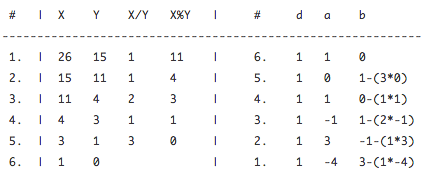
\includegraphics[scale=.45]{gcd.png}
 
 \subsubsection{Fermat's Little Theorem}
 if p is prime, then $\forall$ 1 $\leq$ a $\textless$ p\\
\hspace{5pt} a$^{p-1}$ = 1 mod p \\
\textit{\textbf{Proof:}}{\it Start by listing first p-1 positive multiples of a:\\
S = \{a, 2a, 3a, $\cdots$ (p -1)a\}\\
Suppose that {\it r}a and {\it s}a are the same mod p, $\Rightarrow$ {\it r = s} mod p\\
$\therefore$ set S of p-1 multiples of a are distinct and nonzero, that is, they must be congruent to 1, 2, 3, $\cdots$ p-1 after being sorted.\\
Multiply all congruences together and we find
a$\cdot$2a$\cdot$3a$\cdots$(p-1)$\cdot$a = 1$\cdot$2$\cdot$3$\cdots$(p-1) (mod p)
or better, a$^{(p-1)}$(p-1)! = (p-1)! mod p. Divide both side by (p-1)! $\blacksquare$}\\

\subsubsection{Primality Testing}
\begin{flushleft}\vspace{-16pt}\[
\hspace{-50pt}any \ a  \rightarrow a^{N-1} = 1 \ mod \ N {\it ?}
\begin{cases}
	{\it yes} \Rightarrow {\it "prime"}\\
	{\it no} \Rightarrow {\it composite}
\end{cases}
\]
\end{flushleft}
\vspace{-10pt}if N is not prime a$^{N-1}$ = 1 mod N $\leq$ half values of a $\textless$ N

\subsubsection{Lagrange's Prime Theorem}
Let $\pi$(x) be the \# of primes $leq$ x, then\\
$\pi$(x) $\approx$ $\frac{x}{ln(x)}$, or more precisely lim$_{x \rightarrow \infty} \frac{\pi(x)}{(\frac{x}{ln(x)})} = 1$\\

\subsubsection{Modular Exponentiation}
x$^{y}$ mod N $\rightarrow$ start with repeated squaring mod N\\
x mod N $\rightarrow$ x$^{2}$ mod N $\rightarrow$ (x$^{2}$)$^{^{2}}$ $\cdots$ x$^{log_{2}y}$ mod N\\
each step takes O(log$^{2}N)$ times to compute and \\there are log$_{2}$y steps, $\therefore$ $\in$ O(n$^{3}$),\\ where n is the \# of bits in N

\subsubsection{Formal Limit Proof}
\begin{flushleft}\vspace{-16pt}\[
\hspace{-50pt}lim_{n \rightarrow \infty}\frac{f(n)}{g(n)}
\begin{cases}
\hspace{3pt} \geq \ 0 \ {\it (\infty)} \Rightarrow \ f(n) \ \in \ \Omega(g(n))\\
\hspace{3pt} \textless \ \infty \ {\it (0)} \Rightarrow \ f(n) \ \in \ O(g(n))\\
\hspace{3pt} = c_{_{\mid 0 \textless c \textless \infty}} \Rightarrow \ f(n) \ \in \ \Theta(g(n))\\
\end{cases}
\]
\end{flushleft}

\subsubsection{Logarithm Tricks}
log$_{b}x^{p} = plog_{b}x$\\
$\frac{ln(x)}{ln(m)}$ = log$_{m}$x\\
x$^{log_{b}y} = y^{log_{b}x}$\\

\subsubsection{Complexity Hierarchy}
Exponential\\Polynomial\\Logarithmic\\Constant\\

\subsubsection{Master's Theorem}
T(n) = aT($\frac{n}{b}$) + O(n$^{d}$), if a $\textgreater0, b\textgreater 1, d \geq$ 0\\
\begin{flushleft}\vspace{-16pt}
\[
\hspace{-100pt}T(n)=\begin{cases}
	O(n^{d})$ if d $\textgreater$ log$_{b}a\\
	O(n^{d}log_{b}n)$ if d = log$_{b}a\\
	O(n^{log_{b}n})$ if d $\textless$ log$_{b}a\\
            \end{cases}
\]
\end{flushleft}

\subsubsection{Volker Strassen}
\[
X = 
\begin{bmatrix}
    A & B\\
    C & D\\
\end{bmatrix}
\hspace{3pt} \times \hspace{3pt} Y = 
\begin{bmatrix}
    E & F\\
    G & H\\
\end{bmatrix}
= 
\begin{bmatrix}
    AE+BG & AF+BH\\
    CE+DG & CF+DH\\
\end{bmatrix}
\in O(n^{3})
\]
with recurrence T(n)=8T($\frac{n}{2}$)+O(n$^{2}$) but thanks to Stassen... \\
\[XY = 
\begin{bmatrix}
    P_{5}+P_{4}-P_{2}+P_{6} & P_{1}+P_{2}\\
    P_{3}+P_{4} & P_{1}+P_{5}-P_{3}+P_{7}\\
\end{bmatrix}
\]
{\scriptsize P$_{1}$ = A(F-H) \hspace{3pt} P$_{2}$ = (A+B)H \hspace{3pt} P$_{3}$ = (C+D)E \hspace{3pt} P$_{4}$ = D(G-E) \\
P$_{5}$ = (A+D)(E+H) \hspace{3pt} P$_{6}$ = (B-D)(G+H) \hspace{3pt} P$_{7}$ = (A-C)(E+F)}\\\vspace{3pt}
$\in$ O(n$^{log_{2}7}$) $\approx$ O(n$^{2.81}$) with recurrence T(n)=7T($\frac{n}{2}$)+O(n$^{2}$)\\

\subsubsection

% You can even have references
\rule{0.3\linewidth}{0.25pt}
\scriptsize
\bibliographystyle{abstract}
\bibliography{refFile}
\end{multicols}
\end{document}
